\chap{ Finite State Machines}
\section{Part II}
\begin{itemize}
    \item []\textbf{REQUIREMENT}
        \begin{enumerate}
            \item We wish to implement a finite state machine (FSM) that recognizes two specific sequences of applied input symbols, namely four consecutive 1s or four consecutive 0s. There is an input w and an output z. Whenever w = 1 or w = 0 for four consecutive clock pulses the value of z has to be 1; otherwise, z = 0. Overlapping sequences are allowed, so that if w = 1 for five consecutive clock pulses the output z will be equal to 1 after the fourth and fifth pulses.
            \item A state diagram for this FSM is shown in Figure 2. 
                \begin{figure}[h]
                    \centering
                    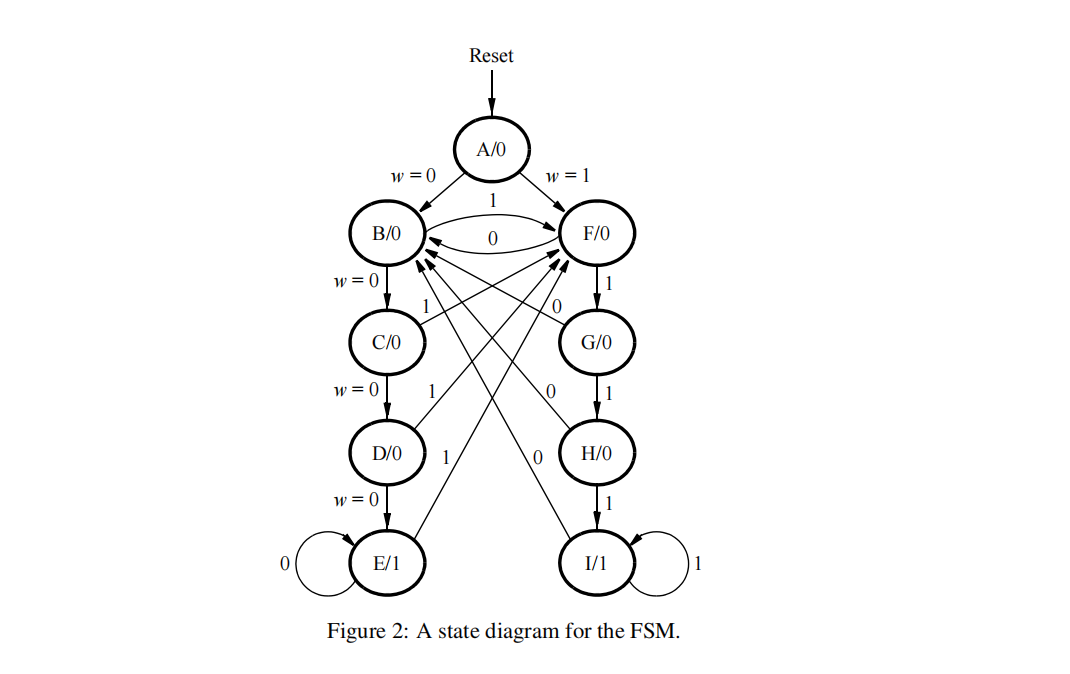
\includegraphics[scale = 0.45]{source/picture/Lab7/minh_hoa_2.png}
                \end{figure}
            \item To implement the FSM use nine state flip-flops called y8, . . . , y0 and the one-hot state assignment given in Table 1.
                \begin{figure}[h]
                    \centering
                    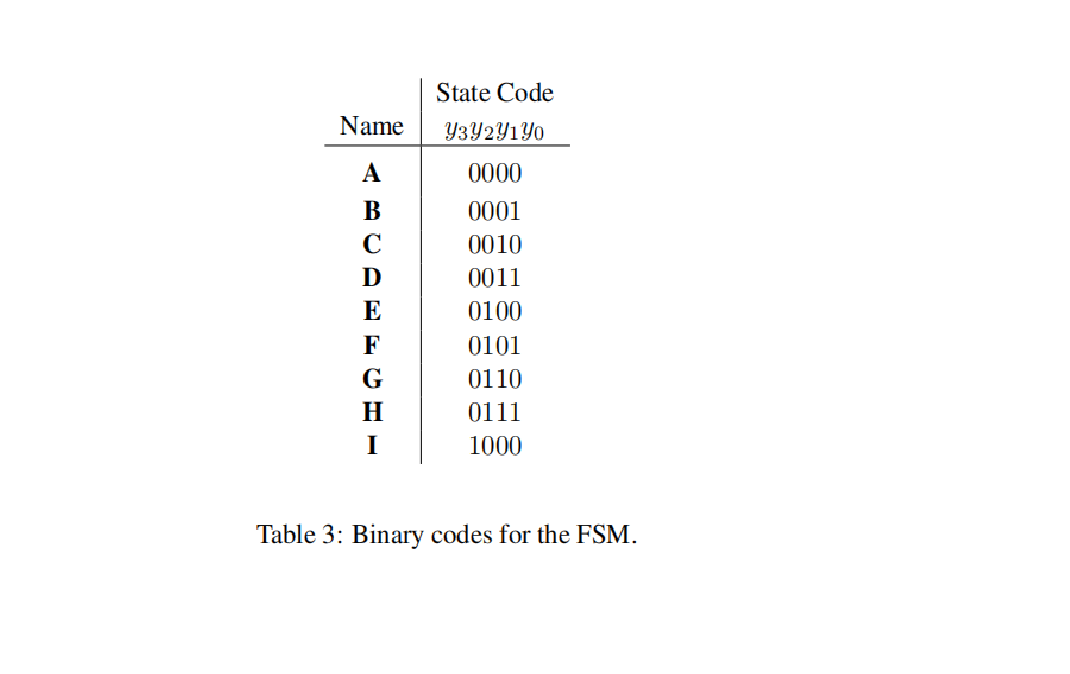
\includegraphics[scale = 0.45]{source/picture/Lab7/minh_hoa_3.png}
                \end{figure}
        \end{enumerate}
\clearpage
    \item []\textbf{SOLUTION}
        \begin{lstlisting}[language=Verilog]
module part2(CLK, RESET, IN, OUT, STATE);
	input		CLK, RESET, IN;
	output	OUT;
	output	[8:0]STATE;
	
	reg		[3:0]YQ, YD;
	parameter 	A = 4'b0000, 
                B = 4'b0001, 
                C = 4'b0010, 
                D = 4'b0011, 
                E = 4'b0100, 
                F = 4'b0101, 
                G = 4'b0110, 
                H = 4'b0111, 
                I = 4'b1000;
	
	always @(IN, YQ) begin
		case (YQ)
			A: begin if (IN) YD = F; else YD = B; end
			B: begin if (IN) YD = F; else YD = C; end
			C: begin if (IN) YD = F; else YD = D; end
			D: begin if (IN) YD = F; else YD = E; end
			E: begin if (IN) YD = F; else YD = E; end
			F: begin if (IN) YD = G; else YD = B; end
			G: begin if (IN) YD = H; else YD = B; end
			H: begin if (IN) YD = I; else YD = B; end
			I: begin if (IN) YD = I; else YD = B; end
			default: YD = 4'bxxxx;
		endcase
	end
	
	always @(posedge CLK) begin
		if (RESET) YQ<=YD;
		else YQ<=A;
	end
	
	change_signal inst0 (.in(YQ), .out(STATE));
	assign OUT = (YQ==E) | (YQ==I);
	
endmodule
        \end{lstlisting}
\clearpage
    \item []\textbf{VERIFICATION}
        \begin{figure}[h]
            \centering
            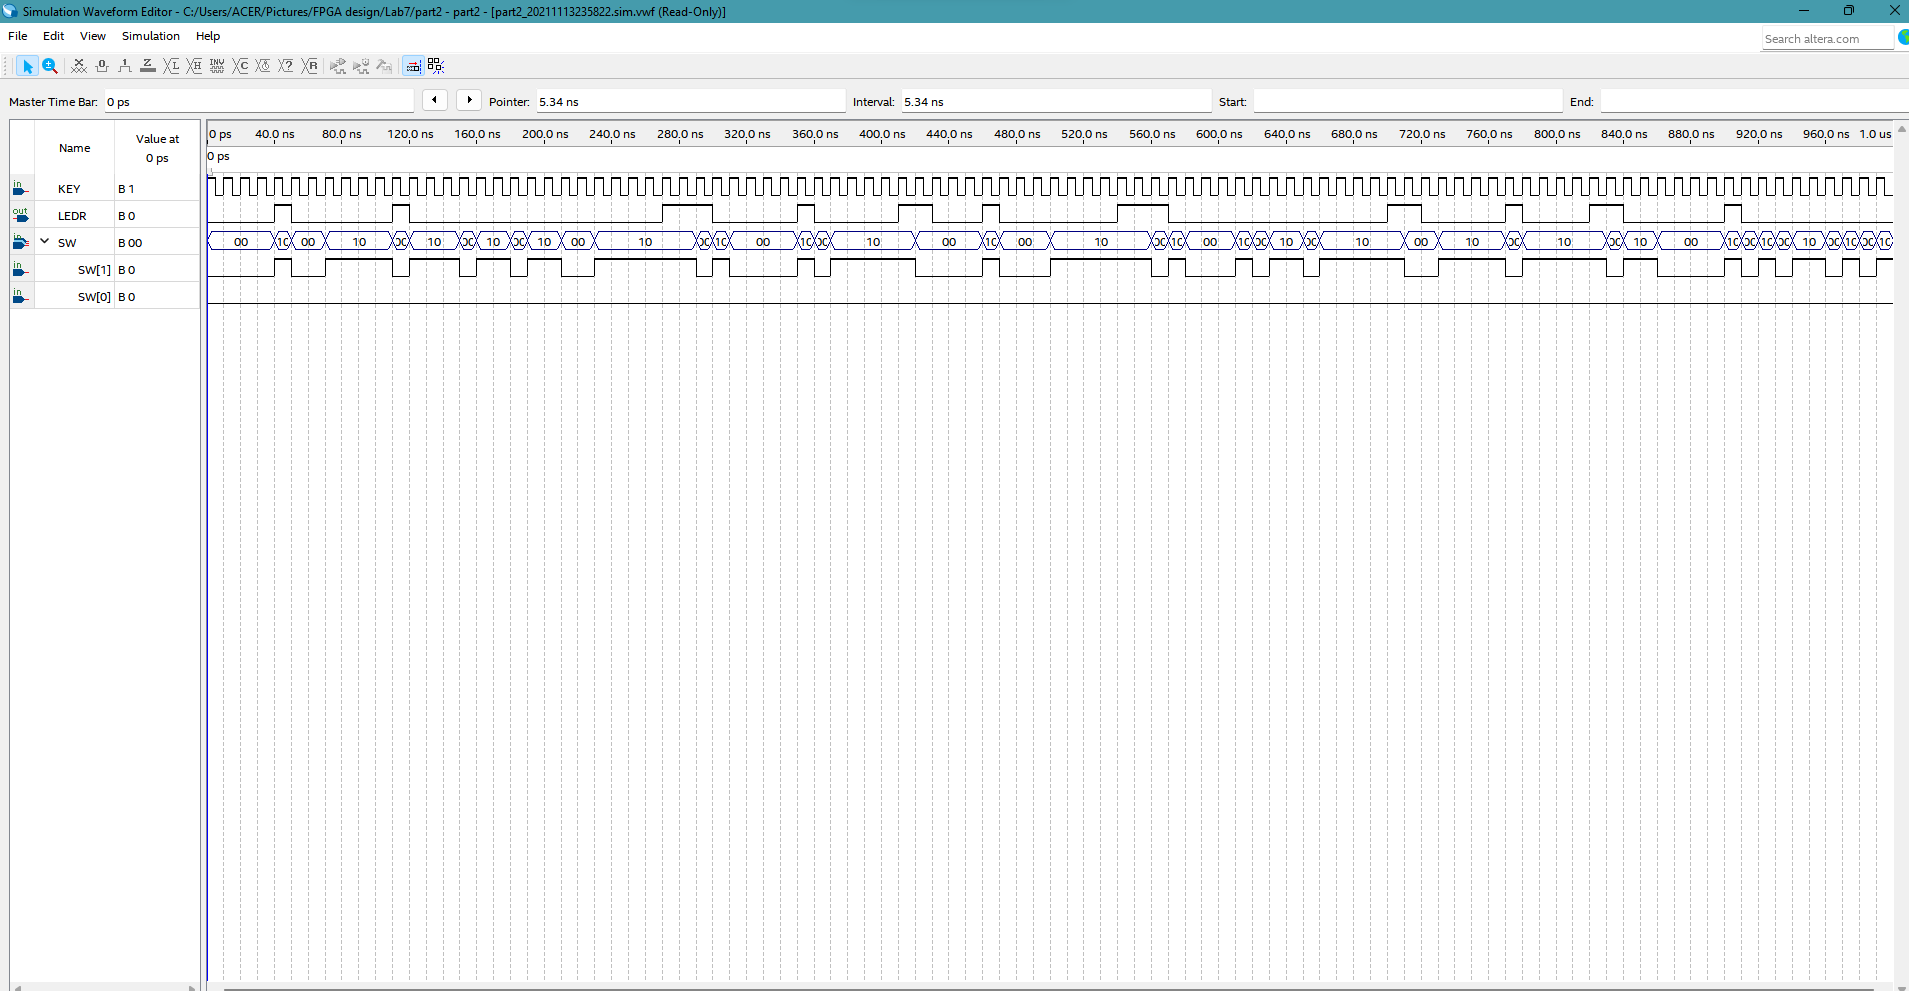
\includegraphics[scale = 0.3]{source/picture/Lab7/bai7_1.png}
            \caption{Simulation Result}
        \end{figure}
\end{itemize}
\newpage



\section{Part IV}
\begin{itemize}
    \item []\textbf{REQUIREMENT}
        \begin{enumerate}
            \item In this part of the exercise you are to implement a Morse-code encoder using an FSM. The Morse code uses patterns of short and long pulses to represent a message. Each letter is represented as a sequence of dots (a short pulse), and dashes (a long pulse). For example, the first eight letters of the alphabet have the following representation:
                \begin{figure}[h]
                    \centering
                    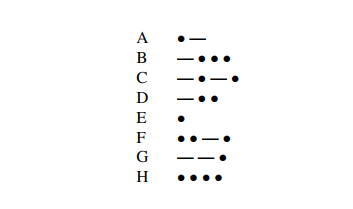
\includegraphics[scale = 0.8]{source/picture/Lab7/Lab7_1.png}
                    \caption{}
                \end{figure}
            \item Design and implement a Morse-code encoder circuit using an FSM. Your circuit should take as input one of the first eight letters of the alphabet and display the Morse code for it on a red LED. Use switches $SW_{2-0}$ and pushbuttons $KEY_{1-0}$ as inputs. When a user presses $KEY_1$, the circuit should display the Morse code for a letter specified by $SW_{2-0}$ (000 for A, 001 for B, etc.), using 0.5-second pulses to represent dots, and 1.5-second pulses to represent dashes. Pushbutton $KEY_0$ should function as an asynchronous reset. 
                \begin{figure}[h]
                    \centering
                    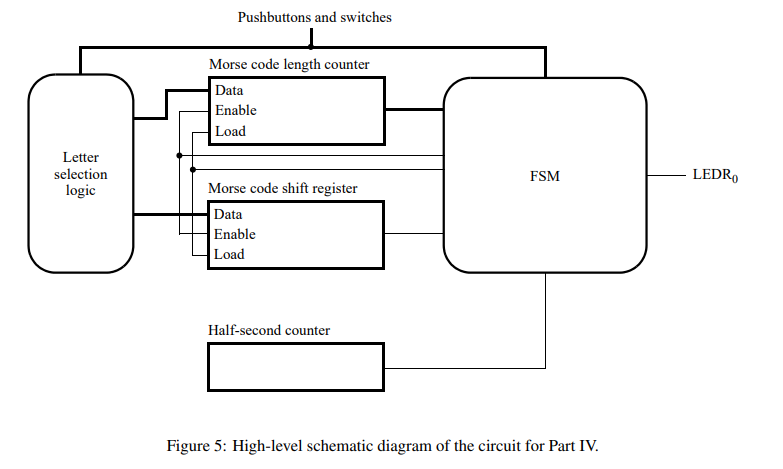
\includegraphics[scale = 0.8]{source/picture/Lab7/Lab7_2.png}
                \end{figure}
        \end{enumerate}
\clearpage

    \item []\textbf{SOLUTION}
        \begin{itemize}
            \item []Our idea is the same with the LAB5\_PART\_IV but now I try to use a state machine so firstly I create state.
                \begin{lstlisting}[language=verilog]
parameter   A=3'b000,
        B=3'b001,
        C=3'b010,
        D=3'b011,
        E=3'b100,
        F=3'b101,
        G=4'b110,
        H=3'b111;
                \end{lstlisting}
            \item []Whenever user change the input I will update the status of the machine
                \begin{lstlisting}[language=verilog]
always@(SW)
begin 
    case(SW)
        A: Y_D=A;
        B: Y_D=B;
        C: Y_D=C;
        D: Y_D=D;
        E: Y_D=E;
        F: Y_D=E;
        G: Y_D=G;
        H: Y_D=H;
    endcase
end
                \end{lstlisting}
            \item []Then when they press button Key\_1 I will update the OUTPUT\_SIGNAL
                \begin{lstlisting}[language=verilog]
always@(posedge KEY[1]) begin
        y_Q = Y_D;
        case (y_Q)
        0: SIGNAL = 14'b00101110000000; // A
        1: SIGNAL = 14'b00111010101000; // B
        2: SIGNAL = 14'b00111010111010; // C
        3: SIGNAL = 14'b00111010100000; // D
        4: SIGNAL = 14'b00100000000000; // E
        5: SIGNAL = 14'b00101011101000; // F
        6: SIGNAL = 14'b00111011101000; // G
        7: SIGNAL = 14'b00101010100000; // H
        default : SIGNAL=14'bxxxxxxxxxxxx;
        endcase
end
                \end{lstlisting}
            \item []The value of Signal have meaning that because I use a counter to count half a second and I will to change the value of LED following the index of SIGNAL ("-"=3'b111=1.5 second, "."=1b'1=0.5 second)
                \begin{lstlisting}[language=verilog]
counter_k_bit ins1(HALFSEC,Clk,KEY[0]);
defparam ins1.n=26;
defparam ins1.k=25000000;//25000000

always @(negedge Clk) begin
    if(HALFSEC==24999999) half=1;//24999999
    else half=0;
end

assign reset=KEY[1] && KEY[0];

counter_k_bit ins2(INDEX,half,reset);
defparam  ins2.n=4;
defparam  ins2.k=14;

always begin
   case (INDEX)
          0:LEDR = SIGNAL[13];
          1:LEDR= SIGNAL[12];
          2:LEDR= SIGNAL[11];
          3:LEDR= SIGNAL[10];
          4:LEDR= SIGNAL[9];
          5:LEDR= SIGNAL[8];
          6:LEDR= SIGNAL[7];
          7:LEDR= SIGNAL[6];
          8:LEDR= SIGNAL[5];
          9:LEDR= SIGNAL[4];
          10:LEDR= SIGNAL[3];
          11:LEDR= SIGNAL[2];
          12:LEDR= SIGNAL[1];
          13:LEDR= SIGNAL[0];
    endcase
end
                \end{lstlisting}
        \end{itemize}
    \item []\textbf{VERIFICATION}
        \begin{figure}[h]
            \centering
            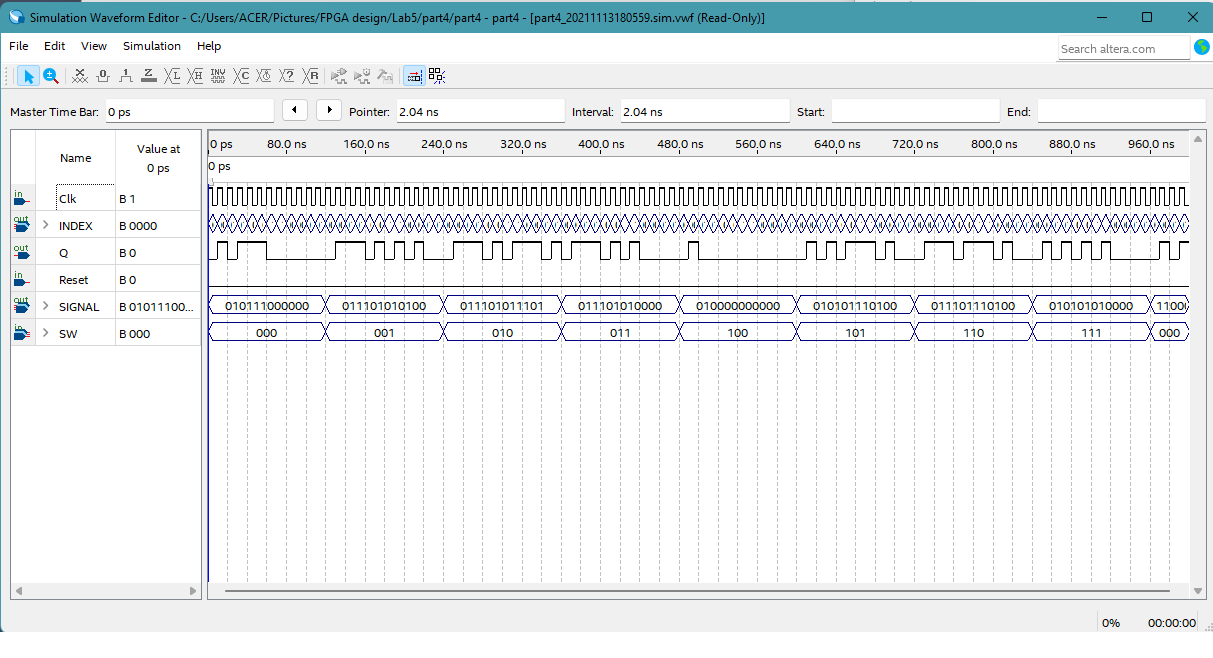
\includegraphics[scale = 0.5]{source/picture/Lab7/bai7.png}
            \caption{Simulation result}
        \end{figure}
\end{itemize}

\clearpage